\tikzstyle{label} = [rectangle, rounded corners, minimum width=1cm, minimum height=0.5cm,text centered, draw=black, fill=red!30]
\begin{frame}{Macrostates and Microstates}
\begin{tikzpicture}[scaleall=1.0,node distance=3cm]]
\node (pic) [] {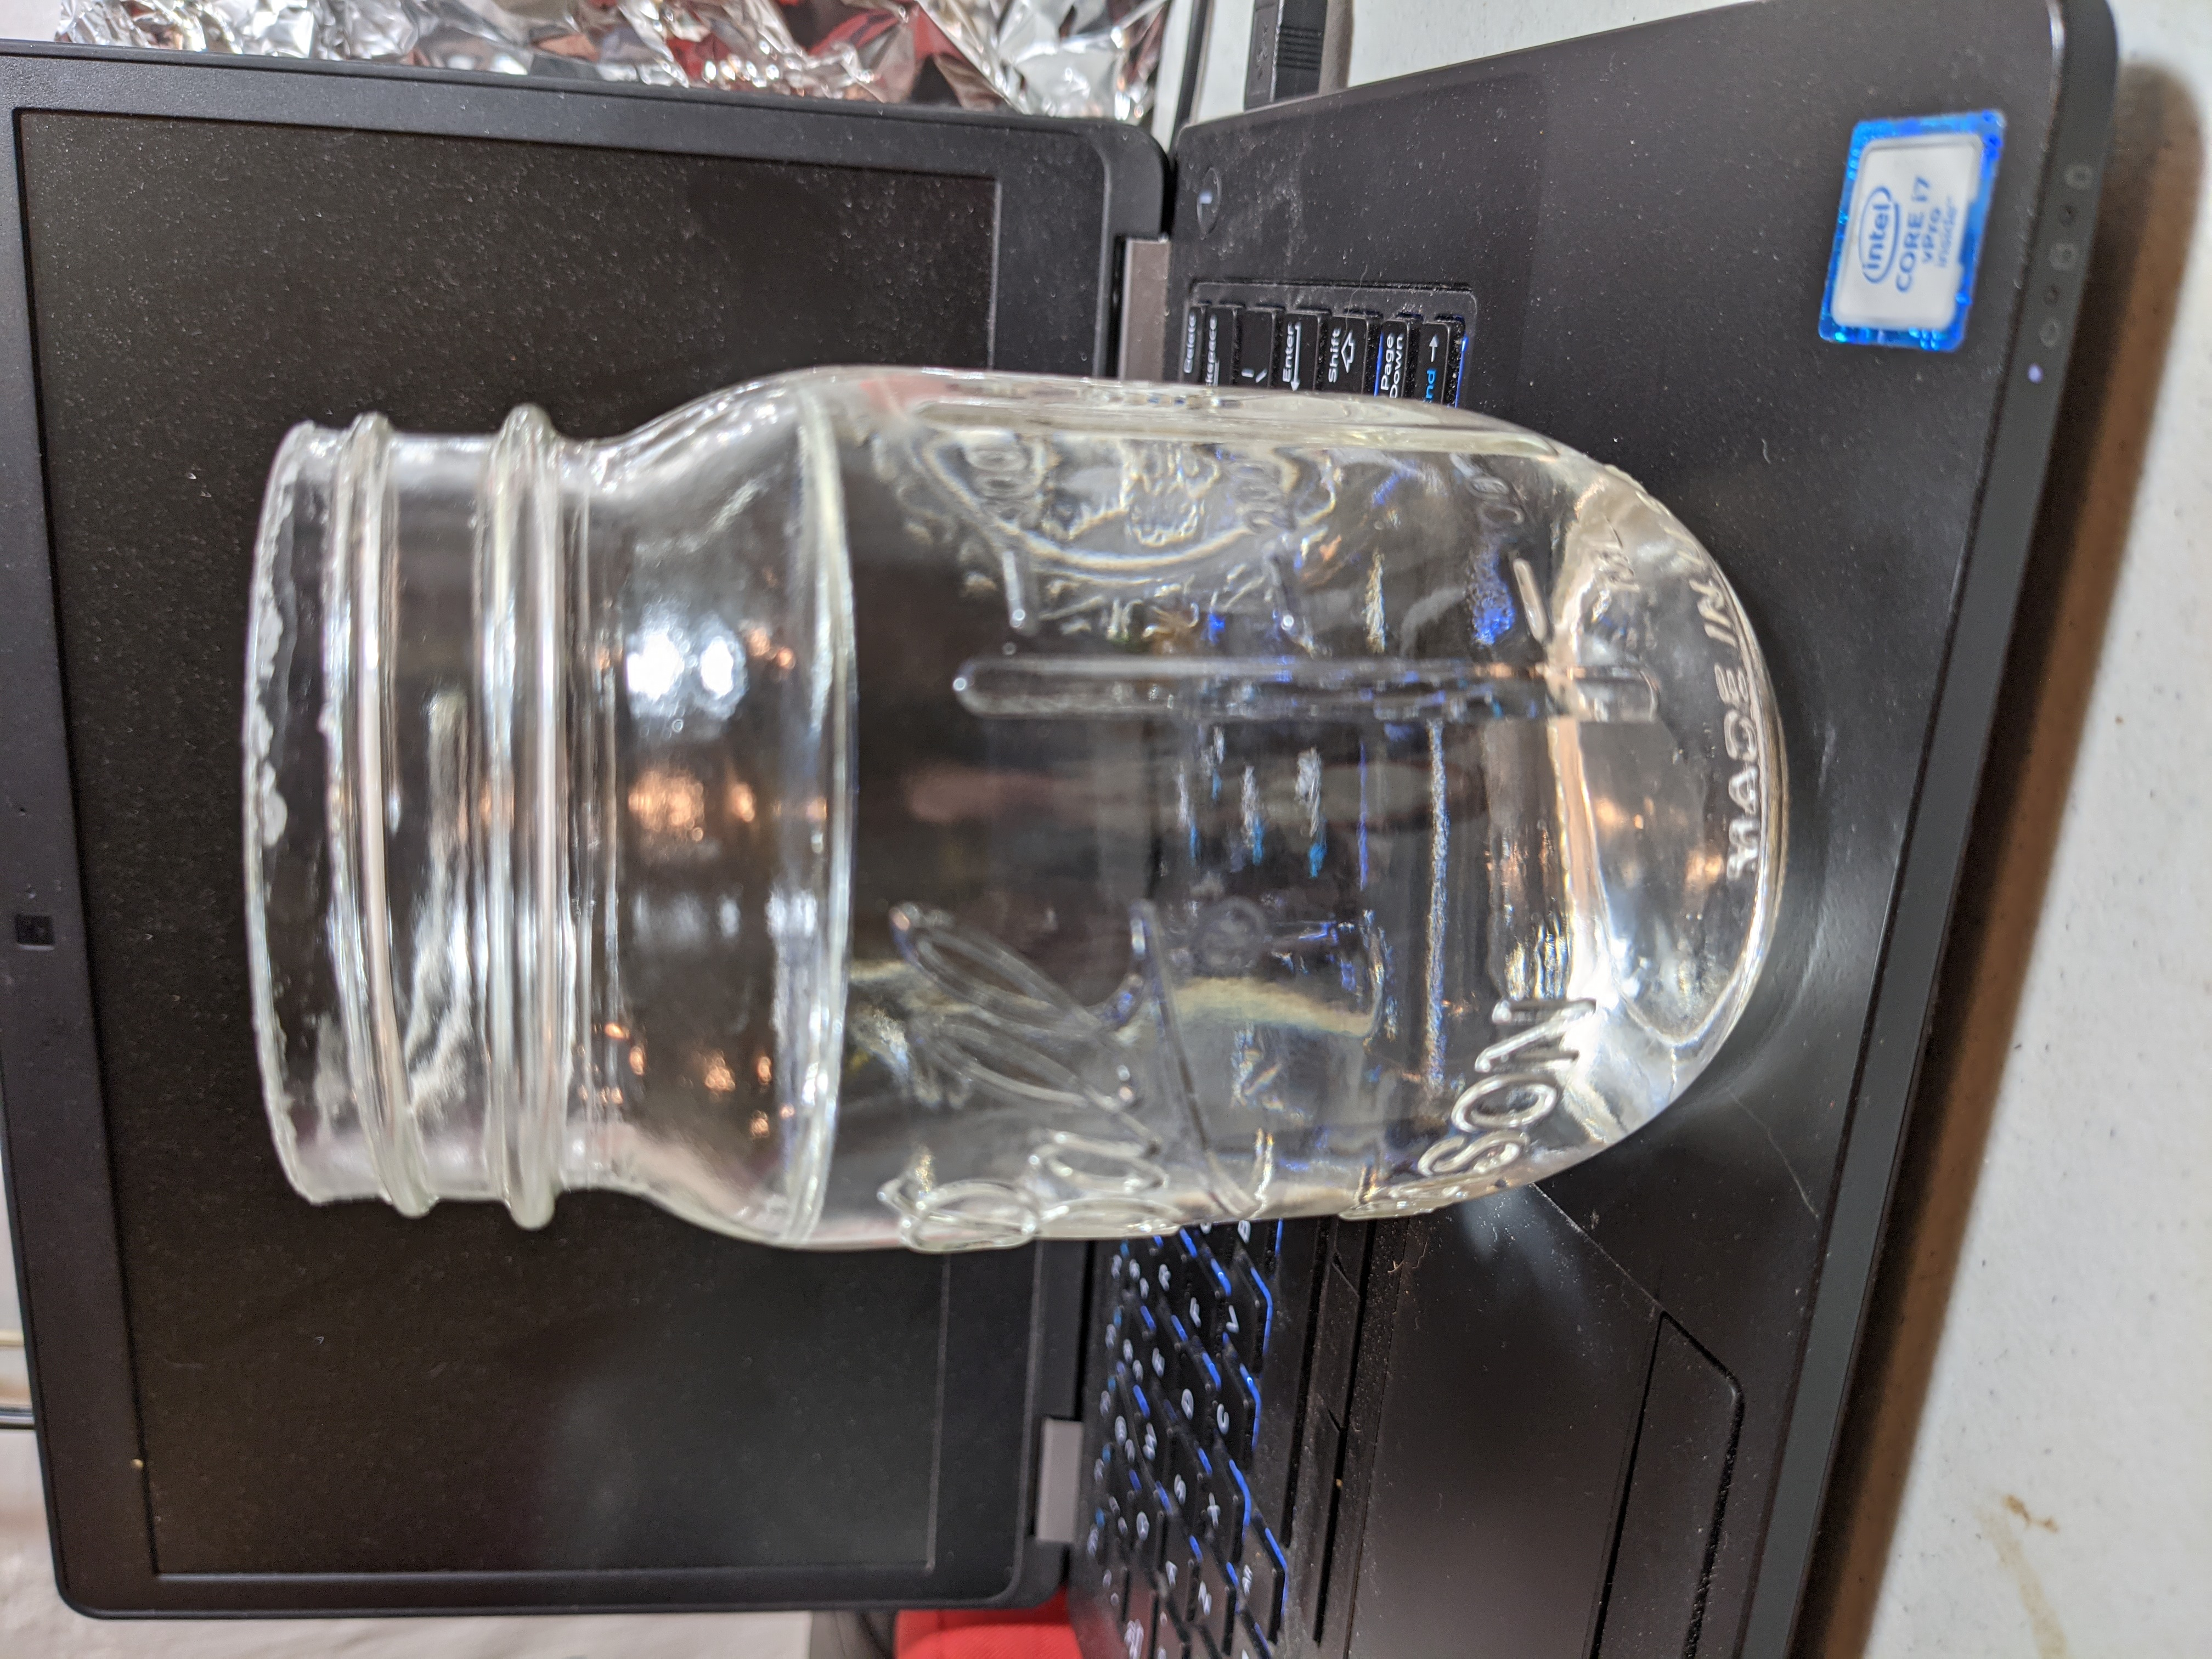
\includegraphics[angle=270,width=0.4\textwidth]{water-pic.jpg}};
\node (label1) [label,below of=pic,yshift=-1cm] {Macrostate}; 
\node (graphic1) [right of=pic,xshift=3cm,yshift=-0.1cm] {
        \animategraphics[loop,controls,width=0.5\textwidth]{10}{movie-water-md/water.000}{00}{90}
    };
\node (label2) [label,below of=graphic1,yshift=-0.9cm] {Microstates (MD)}; 
\end{tikzpicture}
\end{frame}